\section{Query Optimization}
\label{sec:opt}
\name tunes system configurations and optimize complex spatial queries
automatically to make the best use of existing indexes and
statistics. We employed a cost model for determining a proper number
of partitions in different query plans. We also added {\em new logical
  optimization rules} and {\em cost-based optimizations} to the
catalyst optimizer and the physical planner in Spark SQL.

Number of partitions plays an important role in performance tuning in
Spark.  A good choice on the number of partitions not only guarantees
no crashes caused by memory overflow, but also improves throughput and
reduces latency. Given the memory available on a worker node in the
cluster and the input data size, \name partitions the data such that
each partition has roughly equal number of records and they fit into
the memory size of a worker node. This ensures load balancing in the
cluster.

% In \name, we build a cost model to estimate the partition size under a
% schema. It handles two cases: tables with fixed length records and
% tables with varible length record. The first case is simple to
% handle. The cost model estimates the size of a partition based on
% record size $z$, number of records ($m$) that goes into a partition
% (once given a partition strategy), and an estimation of the index size
% (calculated based on the values of $z$ and $m$, and the index type).
% The variable length record case is much harder, since it is difficult
% to estimate the size of a partition even if we know how many recrods
% are going into a partition (e.g., say we have used an equi-depth
% partition strategy to partition the table using a nubmer of quantile
% values so that each partition has roughly same number of records). It
% is also difficult to estimate the size of an index in this
% case. Currently, \name resolves this challenge using a sampling based
% approach, but there is no formal guarantees that the samples will
% always lead to good partitions in the end over the original data.

% Using the cost model and a specified partition strategy, \name then
% computes a good value for the number of partitions such that: 1)
% partitions are balanced in size; 2) size of each partition fits the
% memory size of a worker node; and 3) the total number of partitions is
% proportional to the number of workers in the cluster.  Note that the
% size of a partition should be close but not greater than a threshold,
% which indicates how much heap memory Spark can reserve for query
% processing. In Spark, on each slave node, a fraction of memory is
% reserved for RDD caching, which is specified as a system configuration
% \texttt{spark.storage.memoryFraction} (we denote this value as
% $\alpha$). In our cost model, the remaining memory will be evenly
% split to each processing core. Suppose the number of cores is $c$ and
% total memory reserved for Spark on each slave node is $M$. The
% partition size threshold $\beta$ is then calculated as:
% $\beta =\lambda ((1-\alpha) M / c) $, where $\lambda$ is a system
% parameter, whose default value is 0.8, to take memory consumption of
% run-time data structures into consideration.  With the cost model,
% \name can determine the number of records for a single partition, and
% the numbers of partitions for different data sets.

To better utilize the index support in \name, we add new rules in the
catalyst optimizer to select those predicates which can be optimized
by indexes. First, we transform the original select condition to {\em
  Disjunctive Normal Form} (DNF), e.g.
$(A \wedge B) \vee C \vee (D \wedge E \wedge F)$.  Then, we get rid of
all predicates in the DNF clause which cannot be optimized by indexes
to form a new select condition $\theta$. \name will filter the input
relation with $\theta$ first using index-based operators, and then
apply the original select condition to get the final answer.

% get the final results. We term this procedure as indexed table scan
% optimization.

\begin{figure}[t!]
	\centering
	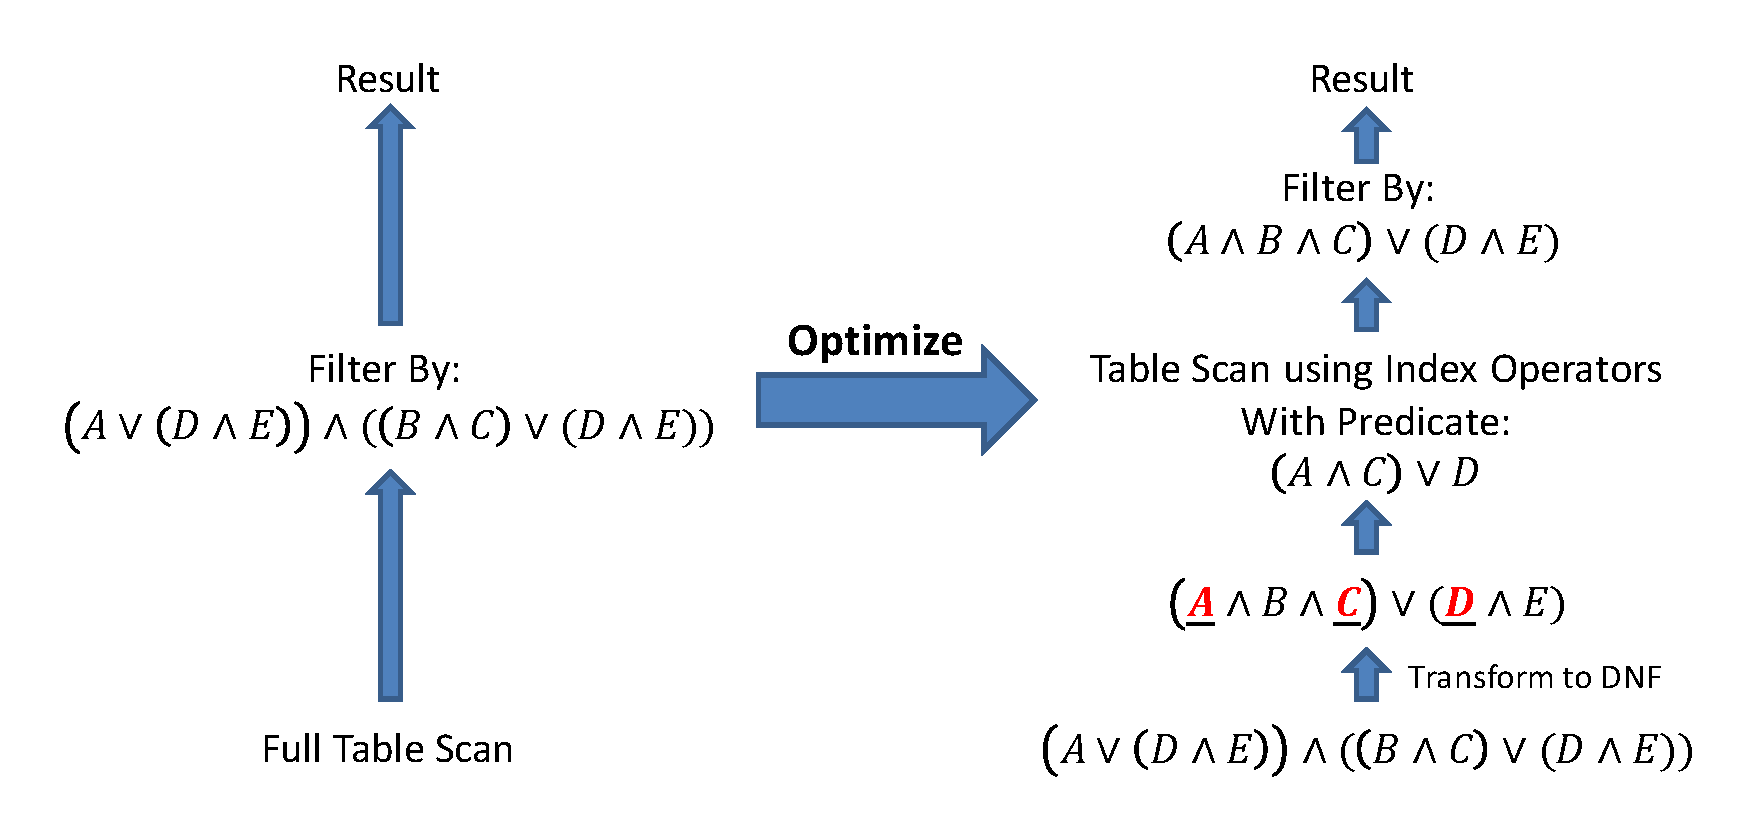
\includegraphics[width=3.4in]{figs/optimize}
	\vspace{-8mm}
	\caption{Index scan optimization in \name.}
	\label{fig:optimize}
	\vspace{-4mm}
\end{figure}

Figure \ref{fig:optimize} shows an example of the index scan
optimization. The select condition on the table is
$(A \vee (D \wedge E)) \wedge ((B \wedge C) \vee (D \wedge E))$.
Assuming that $A$, $C$ and $D$ can be optimized by utilizing existing
indexes. Without index optimization, the engine (e.g., Spark SQL)
simply does a full scan on the table and filters each record by the
input select condition. By applying index optimization, \name works
out the DNF of select condition, which is
$(A \wedge B \wedge C) \vee (D \wedge E)$, and invokes a table scan
using index operators under a new condition $(A \wedge C) \vee D$.
Then, we filter the resulting relation with original condition once
more to get the final results.

\name also explores various {\em geometric properties} to merge
spatial predicates in order to reduce the number of physical
operations. Generally, we merge predicates on single dimension into
segments or bounding boxes, which can be processed together without
involving expensive intersections or unions on intermediate
results. For example, \texttt{x > 3 AND x < 5 AND y > 1 AND y < 6} can
be merged into a range query on \texttt{(POINT(3, 1), POINT(5, 6))},
which is natively supported in \name as a single range query. \name
also merges query segments or bounding boxes prior to execution, so
that it greatly reduces the number of operations. For instance, two
conjunctive range queries on \texttt{(POINT(3, 1), POINT(5, 6))} and
\texttt{(POINT(4, 0), POINT(9, 3))} can be merged into a single range
query on \texttt{(POINT(4, 1), POINT(5, 3))}.

Index optimization improves performance greatly when the predicates
are selective.  However, it may cause more overheads than savings when
query selectivity is low or the size of input table is small. Thus,
\name also uses a new cost based optimization (CBO), which takes
existing indexes and statistics into consideration, to choose the most
efficient physical plans on the fly. Specifically, \name will estimate
the query selectivity using indexes and simple statistics on
tables. % issue a fast partial query to existing indexes so as to get an
% upper bound of condition selectivity. Besides, it will check the
% size of input relation.
If query selectivity is low or the size of input relation is small,
\name will scan the table without utilizing indexes.

CBO is also used for joins in \name. When one of the tables in the
join is small (much smaller compared to the other table), \name's
optimizer will switch to a {\em broadcast join} algorithm by skipping
the data partition phase on the small table, and broadcast the small
table to every partition of the large table to do local joins. For
example, if $R$ is small and $S$ is big, \name will do local joins
over $(R, S_1), \ldots, (R, S_m)$. This applies to both distance and
$k$NN joins.


For $k$NN joins in particular, CBO is used to do fine-tuning for the
RKJ-Spark algorithm. We can increase the sampling rate used to
generate $S'$ and/or partition table $R$ with finer granularity, to
get a tighter bound for $\gamma_i$. \name's optimizer adjusts the
sampling rate of $S'$ according to the memory size on the master node
(and the max possible query value $k_{\max}$ so that $|S'|>k_{max}$;
typically $k$ is small for $k$NN queries). \name's optimizer can also
invoke another STR partition {\em within each local partition} to get
partition boundaries {\em locally on each worker} with finer
granularity without changing the global partition and physical data
distribution. This allows RKJ-Spark to compute tighter bound for
$\gamma_i$ using the refined partition boundaries, thus reduce the
size of $S_i$'s.


Lastly, \name uses a SQL context that is thread-safe (using
thread-local instances for conflicts) to support the execution of
multiple queries concurrently, hence, multiple users can issue queries
concurrently to the same \name instance.


% In Spark 1.3.0 (which is the base system of SparkSpatial), SQL
% context cannot support multiple queries concurrently, as numbers
% of components (e.g. SQL parser, catalyst optimizer) in Spark SQL
% are not thread-safe. To address this problem, SparkSpatial sepa-
% rates such conflict components into thread-local instances. As a re-
% sult, multiple users can now issue queries concurrently to the same
% SparkSpatial instance.

% \SparkSpatial is able to optimize complex queries automatically to
% make the best use of existing table indexes and statistics. We
% extend the catalyst optimizer and the physical planner of Spark SQL
% with new rules to dig out more possibilities for optimizations
% brought by table indexing.

% With the help of table indexes, plenty of operations can achieve
% orders of magnitude better performance than that in the non-index
% cases. \SparkSpatial picks the predicates that can be optimized by
% leveraging table indexes from the original query condition and
% processes them first to shrink the data size as soon as
% possible. Specifically, we first transform the original query
% condition to \emph{Disjunctive Normal Form} (DNF) and select the
% predicates that can be accelerated by existing indexes. Then, we
% only keep the selected predicates in DNF as a new query condition
% and use index-version algorithms (implemented in
% \texttt{IndexRelationScan}) to filter the original data set. To get
% the final result, \SparkSpatial processes the original condition
% once again on the filtered data. This time, it will be much more
% efficient since data size shrinks dramatically in the last step.

% For instance, $A, B, C, D, E$ are predicates from the original query
% condition and DNF of this condition is $(A \wedge B \wedge C) \vee
% (D \wedge E)$. Assuming that $A$, $C$ and $D$ can be optimized by
% utilizing existing indexes, we process $(A \wedge C) \vee D$ in
% \texttt{IndexRelationScan} first to shrink the data size. Next, $(A
% \wedge B \wedge C) \vee (D \wedge E)$ is applied on the shrunk data
% so as to get the final results.

% In addition to optimize query conditions with existing indexes,
% \SparkSpatial also merges predicates to reduce the number of
% physical operations. For example, \texttt{x > 3 AND x < 5 AND y > 1
% AND y < 6} can be merged as a single spatial predicate \texttt{(x,
% y) in RANGE(POINT(3, 1), POINT(5, 6))}, which can be optimized as a
% box range query when there is an R-Tree index built on attribute
% \texttt{x} and \texttt{y}.

% In Spark 1.3.0 (base system of \SparkSpatial), numbers of components
% (e.g. SQL Parser, catalyst optimizer) in Spark SQL are not thread
% safe, which makes Spark SQL unable to support concurrent query
% perfectly. We address this issue by separating these conflict
% components into thread-local instances. Thus, \SparkSpatial can
% support concurrent queries issued by multiple users in the same
% \SparkSpatial instance.


%%% Local Variables:
%%% mode: latex
%%% TeX-master: "paper"
%%% End:
